% \chapter{SVD Analysis of $\mathrm{[Fe^{II}(bpy)_3](PF_6)_2}$ TA Data}
\chapter{SVD Analysis of [Fe\textsuperscript{II}(bpy)\textsubscript{3}](PF\textsubscript{6})\textsubscript{2} TA Data}
\label{ap: sco-bpy}

% Figure: aqueous SVD analysis
\begin{figure}[hp]
  \centering
  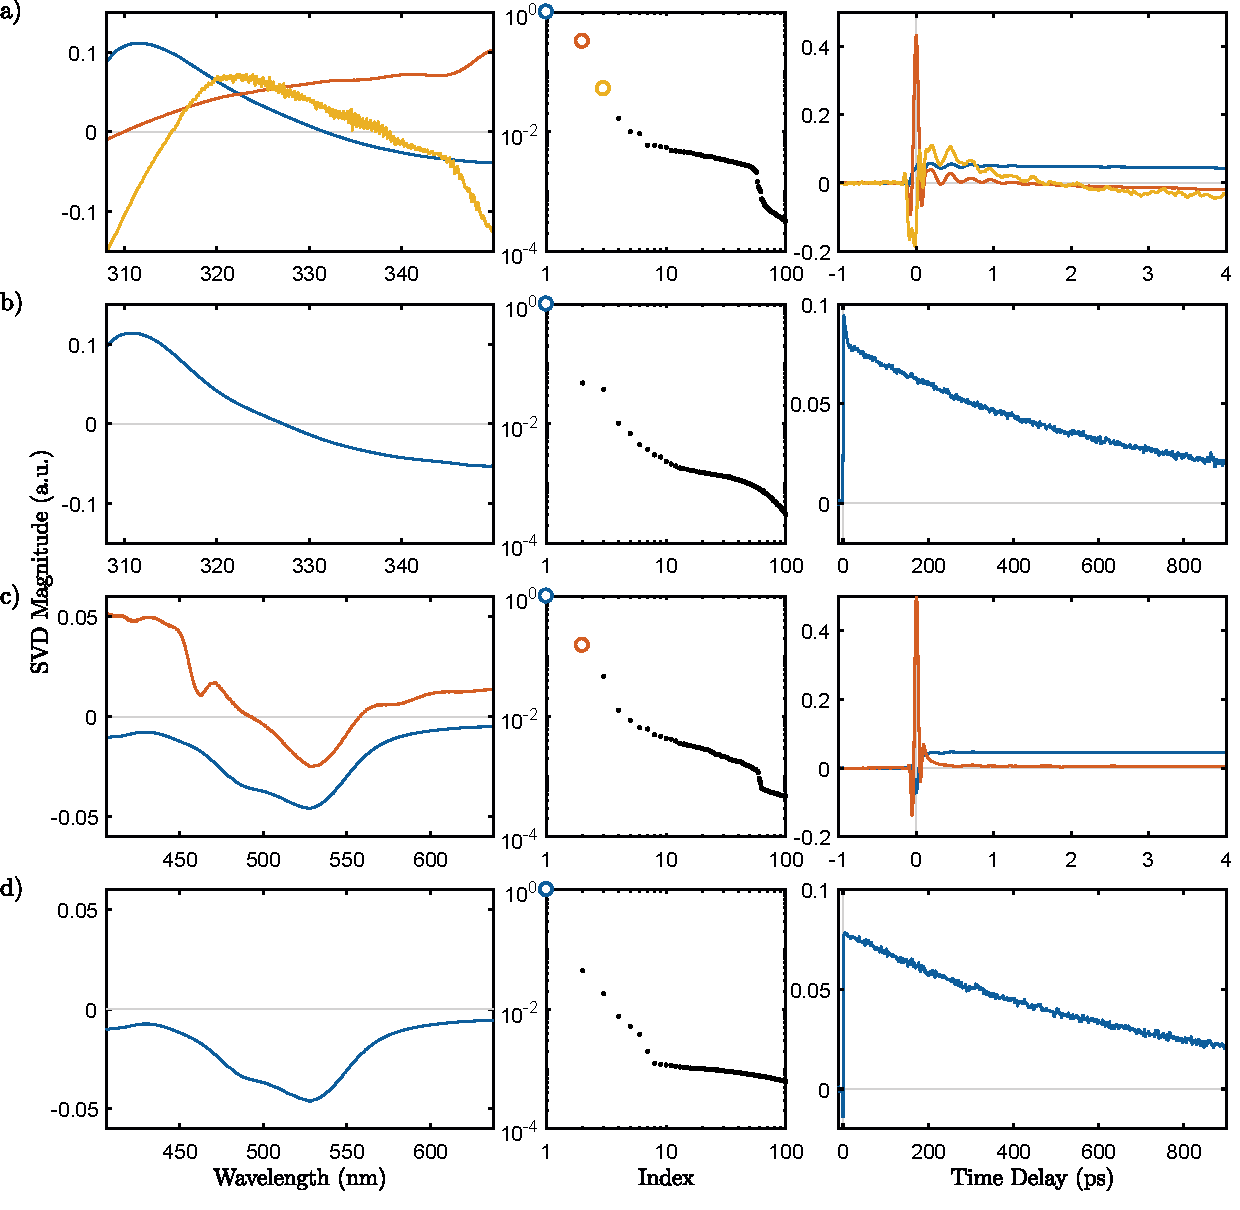
\includegraphics[width = \textwidth]{Figures/fig_BPY_data_aqueous_svd.pdf}
  \caption[SVD analysis of solvated BPY TA data.]{
    SVD analysis of solvated BPY TA data:
    (a) UV short-time, (b) UV long-time, (c) Vis short-time, and (d) Vis long-time.
    From left to right, the panels show
    the principal wavelenght-dependent singular vectors~$u_i(\lambda)$,
    the first 100 singular values~$s_i$,
    and the principal time-dependent singular vectors~$v_i(t)$.
  }
  \label{fig: BPY-data-aqueous-svd}
\end{figure}

% Figure: aqueous SVD analysis
\begin{figure}[p]
  \centering
  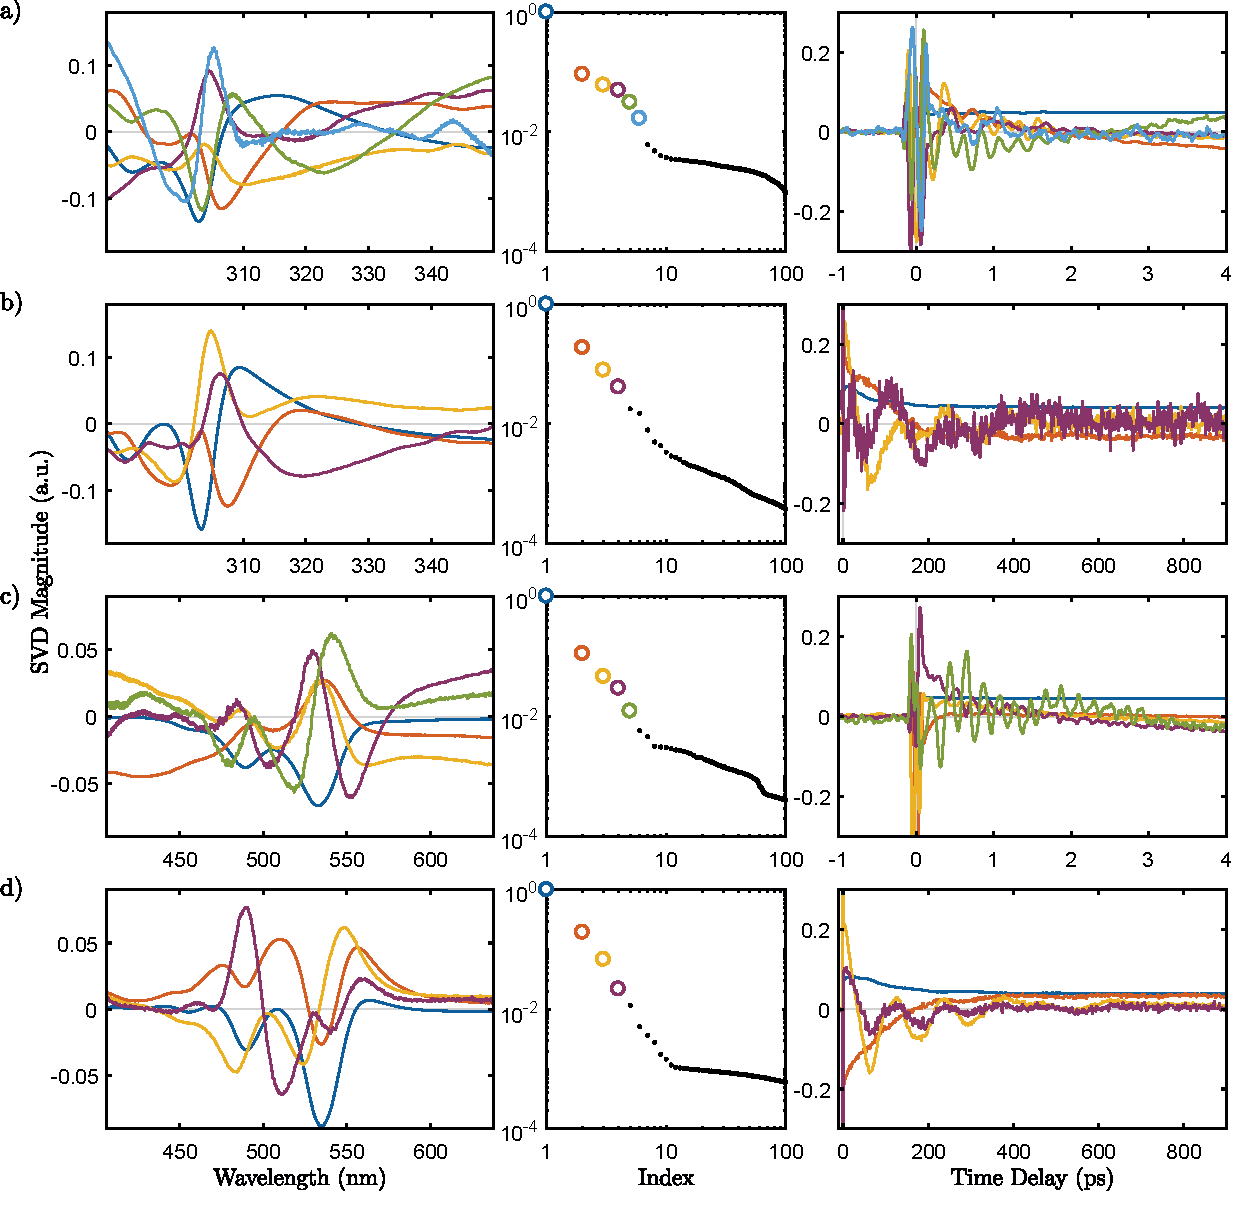
\includegraphics[width = \textwidth]{Figures/fig_BPY_data_crystal_svd.pdf}
  \caption[SVD analysis of single-crystal BPY TA data.]{
    SVD analysis of single-crystal BPY TA data:
    (a) UV short-time, (b) UV long-time, (c) Vis short-time, and (d) Vis long-time.
    From left to right, the panels show
    the principal wavelenght-dependent singular vectors~$u_i(\lambda)$,
    the first 100 singular values~$s_i$,
    and the principal time-dependent singular vectors~$v_i(t)$.
  }
  \label{fig: BPY-data-crystal-svd}
\end{figure}
